\section{CHP Plant}
\label{plant}

Figure \ref{figplant} depicts a schematic of the CHP plant used in this paper. The plant is located in Monz\'on (Huesca), in the north of Spain\footnote{\url{http://www.energyworks.com}}. The main systems of the plant are: four internal combustion engines, four refrigeration engine circuits, an exhaust steam boiler, a steam turbine condenser, a steam turbine, and a slurry drying process. The plant produces electricity by means of the combustion engines and the steam turbine. The steam is generated with the heat contained in the exhaust gases of the four engines. Part of this heat is also used in a slurry drying process being the slurry provided by nearby farms.

\begin{figure}
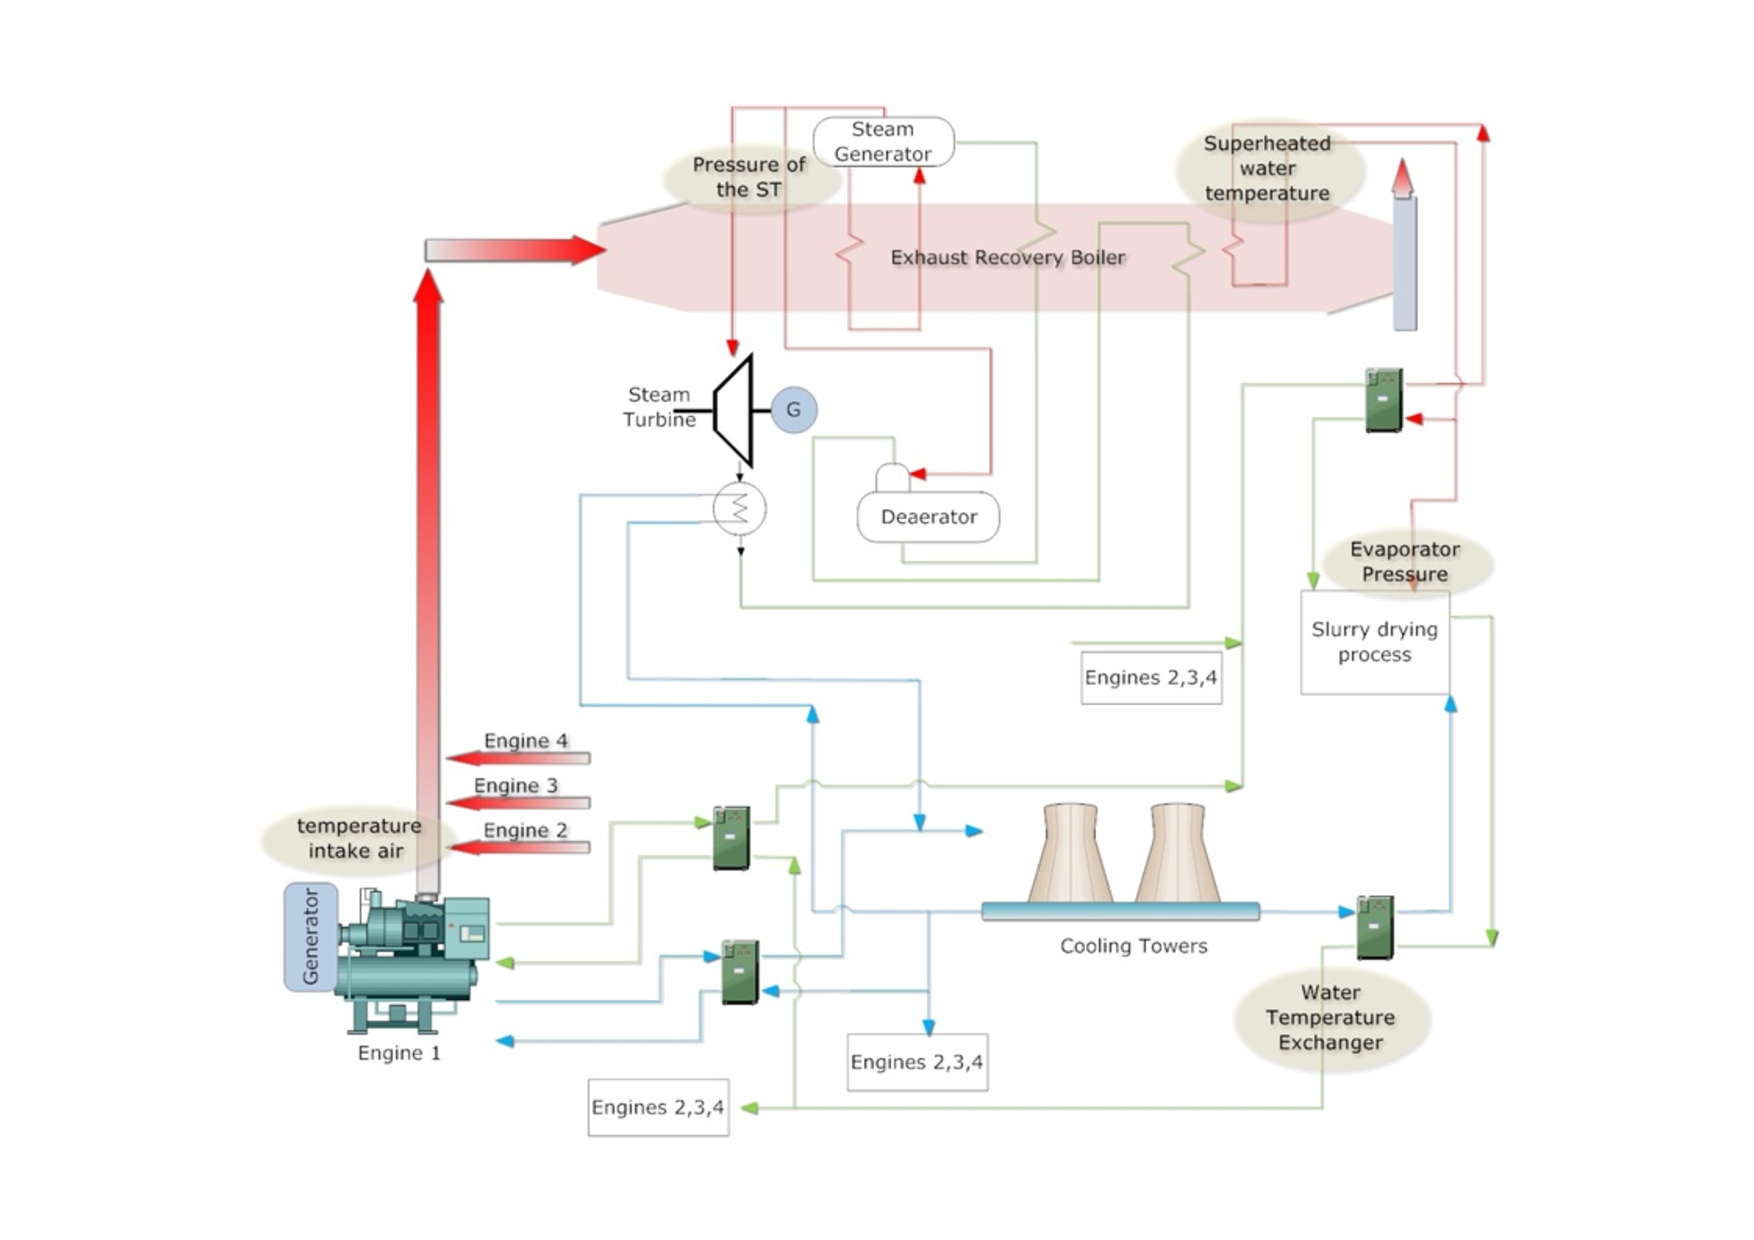
\includegraphics[width=1\textwidth]{plant.pdf}
\caption{Scheme of the combined heat and power process with their related equipment.}
\label{figplant}
\end{figure}

The four internal combustion engines are all identical, with the same characteristics and the nominal power of each being \SI{3700}{kW}. They are organized into two banks with eight cylinders each and the fuel used for the combustion is natural gas. The engines exchange heat with two circuits that use water from the cooling towers, as Figure 1 shows. A cooling circuit refrigerates the mixture of air-fuel around \SI{50}{\celsius} and the other circuit preheats the intake air to around \SI{35}{\celsius}. The engines generate electrical energy, which is sold,  and also flue gases. Each engine has a diverter which sends the flue gases to an exhaust steam boiler when the engine is working above \SI{50}{\percent} of rated power, or to the chimney if the rated power is below \SI{50}{\percent}. Engines are usually above this threshold, and therefore the flue gases go to the exhaust steam boiler most of the time. 

Next, the heat from the exhaust steam boiler is used by the steam generator to create steam around \SI{400}{\celsius} at \SI{22.5}{bar}. This steam feeds the steam turbine to generate more electricity, with \SI{1000}{kW} of nominal power. The condenser of the steam turbine uses water from the cooling towers to condensate the steam from the steam turbine and recirculate it to the system. In addition, as in the engines, the power generated with the steam turbine is also sold. 

The slurry from the farms consists of \SI{6}{\percent} solids approximately. Firstly, a mechanical treatment is carried out to remove the solid part from the rest using rotatory equipment. Then, a chemical treatment in the liquid part is performed to remove the chemical load. After that, the heat treatment uses the result of the chemical treatment to separate the condensables from non-condensables in an evaporator using superheated water generated in the exhaust steam boiler (water with a temperature around \SI{120}{\celsius}). A tubular heater is used to recirculate the effluent to the evaporator and preheat it. The tubular heater uses water from the refrigeration circuit, which preheats the intake air of the engines. The non-condensable part goes with the solid part resulting from the mechanical treatment and is sold as fertilizer. The condensable effluent is condensed again with the water from the cooling towers. Finally, the sterilizer uses the heat from the superheated water to purify the condensed effluent, thereby obtaining water suitable for irrigation. 